\documentclass[12pt]{article}
\usepackage{latexsym,amssymb,amsmath} % for \Box, \mathbb, split, etc.
% \usepackage[]{showkeys} % shows label names
\usepackage{cite} % sorts citation numbers appropriately
\usepackage{path}
\usepackage{url}
\usepackage{verbatim}
\usepackage{graphicx}
\usepackage{array}
\usepackage{multirow}

% horizontal margins: 1.0 + 6.5 + 1.0 = 8.5
\setlength{\oddsidemargin}{0.0in}
\setlength{\textwidth}{6.5in}
% vertical margins: 1.0 + 9.0 + 1.0 = 11.0
\setlength{\topmargin}{0.0in}
\setlength{\headheight}{12pt}
\setlength{\headsep}{13pt}
\setlength{\textheight}{625pt}
\setlength{\footskip}{24pt}

\renewcommand{\textfraction}{0.10}
\renewcommand{\topfraction}{0.85}
\renewcommand{\bottomfraction}{0.85}
\renewcommand{\floatpagefraction}{0.90}
\usepackage{graphicx}
\usepackage{wrapfig}
\usepackage{lscape}
\usepackage{rotating}
\usepackage{epstopdf}
\makeatletter
\setlength{\arraycolsep}{2\p@} % make spaces around "=" in eqnarray smaller
\makeatother

% change equation, table, figure numbers to be counted inside a section:
\numberwithin{equation}{section}
\numberwithin{table}{section}
\numberwithin{figure}{section}

% begin of personal macros
\newcommand{\half}{{\textstyle \frac{1}{2}}}
\newcommand{\eps}{\varepsilon}
\newcommand{\myth}{\vartheta}
\newcommand{\myphi}{\varphi}
\usepackage[utf8]{inputenc}

% Default fixed font does not support bold face
\DeclareFixedFont{\ttb}{T1}{txtt}{bx}{n}{8} % for bold
\DeclareFixedFont{\ttm}{T1}{txtt}{m}{n}{8}  % for normal

% Custom colors
\usepackage{color}
\definecolor{deepblue}{rgb}{0,0,0.5}
\definecolor{deepred}{rgb}{0.6,0,0}
\definecolor{deepgreen}{rgb}{0,0.5,0}
\definecolor{backcolour}{rgb}{0.96,0.96,0.96}

\usepackage{listings}

% Python style for highlighting
\newcommand\pythonstyle{\lstset{
		language=Python,
		basicstyle=\ttm,
		otherkeywords={self},             % Add keywords here
		keywordstyle=\ttb\color{deepblue},
		emph={MyClass,__init__},          % Custom highlighting
		emphstyle=\ttb\color{deepred},    % Custom highlighting style
		stringstyle=\color{deepgreen},
		frame=tb,                         % Any extra options here
		showstringspaces=false,            % 
		backgroundcolor=\color{backcolour}
}}


% Python environment
\lstnewenvironment{python}[1][]
{
	\pythonstyle
	\lstset{#1}
}
{}

% Python for external files
\newcommand\pythonexternal[2][]{{
		\pythonstyle
		\lstinputlisting[#1]{#2}}}

% Python for inline
\newcommand\pythoninline[1]{{\pythonstyle\lstinline!#1!}}

\newcommand{\IN}{\mathbb{N}}
\newcommand{\IZ}{\mathbb{Z}}
\newcommand{\IQ}{\mathbb{Q}}
\newcommand{\IR}{\mathbb{R}}
\newcommand{\IC}{\mathbb{C}}
\newcommand{\Real}[1]{\mathrm{Re}\left({#1}\right)}
\newcommand{\Imag}[1]{\mathrm{Im}\left({#1}\right)}
\usepackage{booktabs}
\usepackage{caption}
\usepackage{float}
\usepackage{titlesec}
\usepackage{capt-of}
%dashed line
\usepackage{array}
\usepackage{arydshln}
\setlength\dashlinedash{0.2pt}
\setlength\dashlinegap{1.5pt}
\setlength\arrayrulewidth{0.3pt}

%Widows & Orphans & Penalties

\widowpenalty500
\clubpenalty500
\clubpenalty=9996
\exhyphenpenalty=50 %for line-breaking at an explicit hyphen
\brokenpenalty=4991
\predisplaypenalty=10000
\postdisplaypenalty=1549
\displaywidowpenalty=1602
\floatingpenalty = 20000
\usepackage[T1]{fontenc}
\usepackage{fontspec}
\setmainfont[Scale=0.85, Ligatures={Required,Common,Contextual,TeX}]{TeX Gyre Schola} % Incredible font inside latex


\newcommand{\norm}[2]{\|{#1}\|_{{}_{#2}}}
\newcommand{\abs}[1]{\left|{#1}\right|}
\newcommand{\ip}[2]{\left\langle {#1}, {#2} \right\rangle}
\newcommand{\der}[2]{\frac{\partial {#1}}{\partial {#2}}}
\newcommand{\dder}[2]{\frac{\partial^2 {#1}}{\partial {#2}^2}}
\usepackage{enumitem}
\newcommand{\nn}{\mathbf{n}}
\newcommand{\xx}{\mathbf{x}}
\newcommand{\uu}{\mathbf{u}}
\usepackage{tikz}
\usetikzlibrary{arrows}
\usetikzlibrary{positioning}
\usepackage{titlesec}
\newcommand{\junk}[1]{{}}
\usepackage{sectsty}
\usepackage{xcolor}

\newcommand\MyBox[2]{
	\fbox{\lower0.75cm
		\vbox to 1.7cm{\vfil
			\hbox to 1.7cm{\hfil\parbox{1.4cm}{#1\\#2}\hfil}
			\vfil}%
	}%
}

\makeatletter
\renewcommand*\env@matrix[1][\arraystretch]{%
	\edef\arraystretch{#1}%
	\hskip -\arraycolsep
	\let\@ifnextchar\new@ifnextchar
	\array{*\c@MaxMatrixCols c}}
\makeatother

\makeatletter
\renewcommand*\env@matrix[1][*\c@MaxMatrixCols c]{%
	\hskip -\arraycolsep
	\let\@ifnextchar\new@ifnextchar
	\array{#1}}
\makeatother

\definecolor{darkblue}{rgb}{0,0,0.4}
\usepackage[colorlinks = true,
linkcolor = darkblue,
urlcolor  = darkblue,
citecolor = darkblue,
anchorcolor = darkblue]{hyperref}
% set two lengths for the includegraphics commands used to import the plots:
\newlength{\fwtwo} \setlength{\fwtwo}{0.45\textwidth}
% end of personal macros

\begin{document}
\DeclareGraphicsExtensions{.jpg}

\begin{center}
\textsc{\Huge Data Mining} \\[2pt]
	\textsc{\Large Assignment 3}\\
	\vspace{0.5cm}
  Ali Gholami \\[6pt]
  Department of Computer Engineering \& Information Technology\\
  Amirkabir University of Technology  \\[6pt]
  \def\UrlFont{\em}
  \url{https://aligholamee.github.io}\\
\href{mailto:aligholami7596@gmail.com}{\textit{aligholami7596@gmail.com}}
\end{center}

\begin{abstract}
 Naive Bayes is a family of algorithms based on applying Bayes theorem with a strong(naive) assumption (bias), that every feature is independent of the others, in order to predict the category of a given sample. They are probabilistic classifiers, therefore will calculate the probability of each category using Bayes theorem, and the category with the highest probability will be output. Naive Bayes classifiers have been successfully applied to many domains, particularly Natural Language Processing (NLP).
\end{abstract} 

\subparagraph{Keywords.} \textit{Natural Language Processing, Text Processing, Text Classification, Spam Filter, Naive Bayes Classifier, Weka.}

\section{Text Preprocessing}
\subsection{Separating Train and Test Data}
In the first step, we need to properly separate the train samples and their labels from each other. To achieve this, we have implemented the function \textit{extract labels} to does that for us. Columns are based on the current dataset which is called \textit{spam collection dataset}.

\begin{python}
	def extract_labels(data):
		return (dataset['v2'], data['v1'])
\end{python}

\subsection{Extracting Features of Texts}
In this section, we'll be using \textit{Bag of Words} model from \textit{Scikit-learn} to to turn the text content into numerical feature vectors. This model does the following steps to turn texts into feature maps.
\begin{enumerate}
	\item Assign a fixed ID to every word occurring in any document (for instance by building a dictionary from words to integer indices).
	
	\item Each unique word in our dictionary will correspond to a feature (descriptive feature).
\end{enumerate}
Scikit-learn has a high level component which will create feature vectors for us \textit{CountVectorizer}.
\begin{python}
	count_vect = CountVectorizer()
	X_train = count_vect.fit_transform(train_data)
\end{python}
It worths mentioning that the parameters and return value of the \textit{fit\_transform} function is as follows:
\begin{python}
	Parameters
	----------
	raw_documents : iterable
	An iterable which yields either str, unicode or file objects.
	
	Returns
	-------
	X : array, [n_samples, n_features]
	Document-term matrix.
\end{python}

\subsection{Issue With Occurrences}
Occurrence count is a good start but there is an issue: longer documents will have higher average count values than shorter documents, even though they might talk about the same topics.

To avoid these potential discrepancies it suffices to \textbf{divide} the number of occurrences of each word in a document by the total \textbf{number of words in the document}. We'll delve into the formal representation of the \textit{TF-IDF}. It is a numerical statistic that is intended to reflect how important a word is to a document in a collection or corpus.
\subsubsection{Term Frequency}
We denote the raw count of a word in a document as $f_{t, d}$. It show the number of times that term \textit{t} has occurred in the document \textit{d}. There are also other approaches to denote the number of occurrences of a term in a document and they are trying to illustrate the weighted frequency of each term in a document. Some of them are:
\begin{itemize}
	\item Boolean Frequencies
	\item Logarithmically Scaled Frequency
	\item Augmented Frequencies
\end{itemize}

\subsubsection{Inverse Document Frequency}
The inverse document frequency is a measure of how much information the word provides, that is, whether the term is common or rare across all documents. It is the logarithmically scaled inverse fraction of the documents that contain the word, obtained by dividing the total number of documents by the number of documents containing the term, and then taking the logarithm of that quotient.
$$
	idf(t, D) = \log \frac{N}{|\{d \epsilon D: t \epsilon d\}}
$$
Where N is the number of documents in the database D. The denominator illustrates the number of documents in which they include the term $t$.

\subsubsection{TF-IDF}
A high weight in tf–idf is reached by a high term frequency (in the given document) and a low document frequency of the term in the whole collection of documents.
$$
	tfidf(t, d, D) = tf(t, d) * idf(t, D)
$$

So far we have defined metrics that can be conducted to improve the features extracted from the emails in the first step. We'll change the transformer to use the \textit{tf-idf} metric to extract features. Using this approach will result in a more precise text classification. This will \textbf{normalize the frequency of redundant words}.
\begin{python}
	count_vect = CountVectorizer()
	X_train = count_vect.fit_transform(train_data)
	
	tf_idf = TfidfTransformer()
	X_train = tf_idf.fit_transform(X_train)
\end{python}

\section{Text Classification}
Now that we have our features, we can train a classifier to try to predict the category of a post as \textit{Spam} or \textit{Ham} (Not Spam). There are various algorithms which can be used for text classification. We will start with the most simplest one called Naive Bayes. For this task, we only need the two class Naive Bayes classifier. We have also included the testing section of the code. The result will be available in the \textit{predict} variable.
\begin{python}
	clf = MultinomialNB().fit(train_data, train_labels)
	test_data = count_vect.transform(test_data)
	test_data = tf_idf.transform(test_data)
	print("Accuracy: ", accuracy_score(test_labels, predicted))
\end{python}
In order to use \textit{Recall} and \textit{Precision} metrics of Scikit-learn, we have to convert the labels into binary format. We'll use \textit{Label Binarizer} to achieve this.
\begin{python}
	lb = preprocessing.LabelBinarizer()
	predicted_binarized = lb.fit_transform(predicted)
	test_labels_binarized = lb.fit_transform(test_labels)
	print("Recall: ", recall_score(test_labels_binarized, predicted_binarized))
	print("Precision: ", precision_score(test_labels_binarized, predicted_binarized))
\end{python}
The final scores for this prediction are given below.
\begin{python}
	Accuracy:  0.9623655913978495
	Recall:  0.7307692307692307
	Precision:  1.0
\end{python}


\section{Bonus: Weka Tools}
For the final section of this report, we'll be introducing some useful tools of \textit{Weka} software. 

\subsection{The Labor Dataset}
In the following sections, we'll use the \textit{Labor} dataset.

\subsection{Selecting the Dataset}
To select the Labor dataset, open the \textit{preprocess} tab and select the dataset according to the figure below.
\begin{figure}[!h]
	\centering
	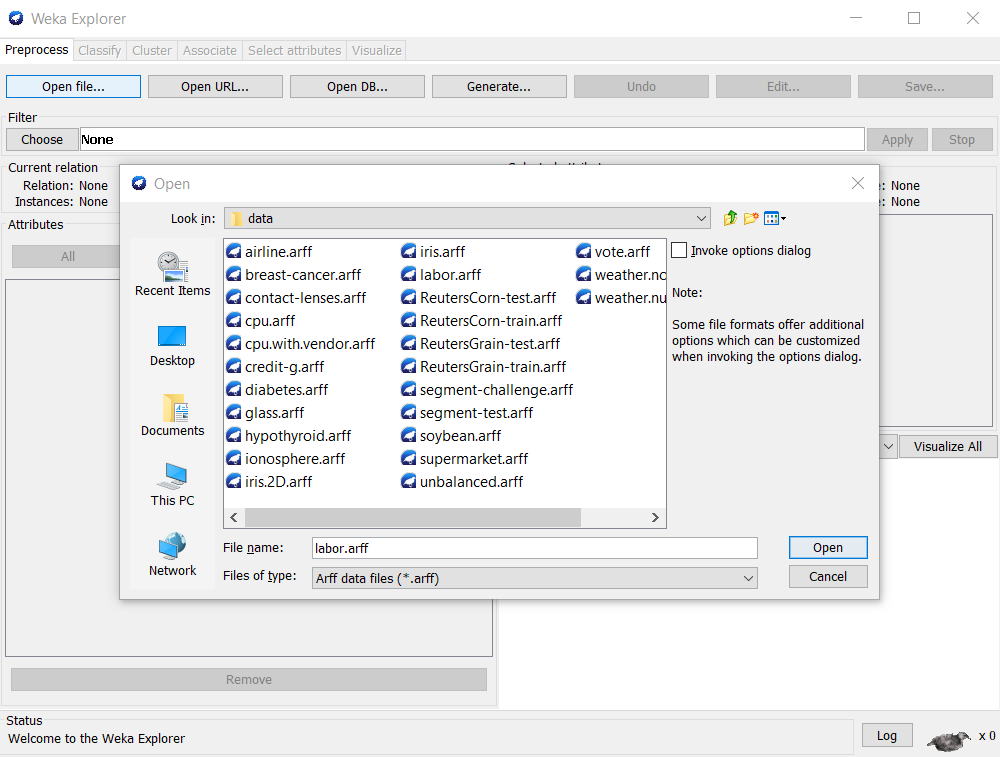
\includegraphics[scale=0.6]{2_1.png}
	\caption{Selecting the proper dataset.}
	\label{fig:PropProf}
\end{figure}

\subsection{Training J48}
Now we open up the \textit{Classify} tab and select the \textit{J48} decision tree classifier from the \textit{trees} section. Here is the performance metrics for this classifier.
\begin{figure}[!h]
	\centering
	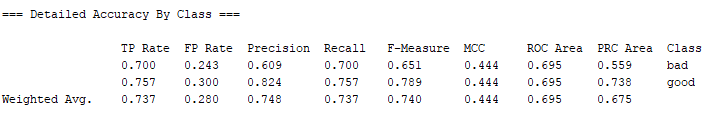
\includegraphics[scale=1]{2_2.png}
	\caption{Performance of J48 on Labor Dataset.}
	\label{fig:PropProf}
\end{figure}
The confusion matrix generated by Weka is also given in the figure 3.3.
\begin{figure}[!h]
	\centering
	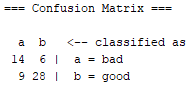
\includegraphics[scale=1]{2_3.png}
	\caption{Confusion Matrix of J48 Classifier on Labor Dataset.}
	\label{fig:PropProf}
\end{figure}

\subsubsection{Precision}
We can use the following formula to compute the \textit{Precision} out of the given confusion matrix. \textit{b} is considered as \textit{positive} and \textit{a} is considered as negative.
$$
	PPV = \frac{TP}{TP + FP} = \frac{28}{28 + 6} = 0.82
$$

\subsubsection{Recall}
We can obtain \textit{Recall} of this classifier using the following formula.
$$
	TPR = Recall = \frac{TP}{TP + FN} = \frac{28}{28 + 9} = 0.75
$$

\subsubsection{F1-Score}
F1-Score can be retrieved as follows. 
$$
	F1_{score} = \frac{2 * PPV * TPR}{PPV + TPR} = \frac{2 * 0.82 * 0.75}{0.82 + 0.75} = \frac{1.23}{1.57} = 0.78
$$

\subsubsection{Decision Tree Visualization}
To visualize the learned decision tree, right click on the item in results list and select the \textit{visualize tree} option.
\begin{figure}[!h]
	\centering
	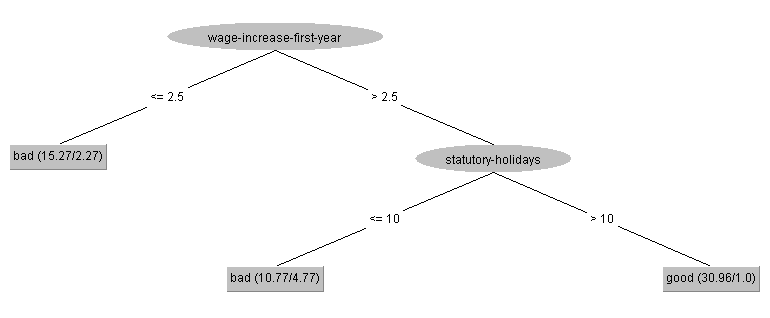
\includegraphics[scale=1]{2_4.png}
	\caption{Visualization of the J48 Decision Tree.}
	\label{fig:PropProf}
\end{figure}

\subsubsection{Testing the Model}
To keep things as simple as possible, test data in the figure 3.5 using the learned tree and find the output label of the model.
\begin{figure}[!h]
	\centering
	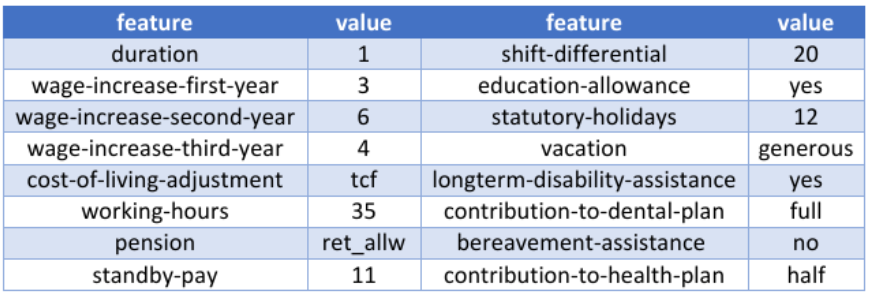
\includegraphics[scale=0.8]{2_5.png}
	\caption{Test Data.}
	\label{fig:PropProf}
\end{figure}

The proper label will be \textit{good}. Note that we have used the product of sum of the tree attributes to find the proper label.

\subsection{Training with Decision Stump}
The same evaluation results is given in the figure 3.6.

\begin{figure}[!h]
	\centering
	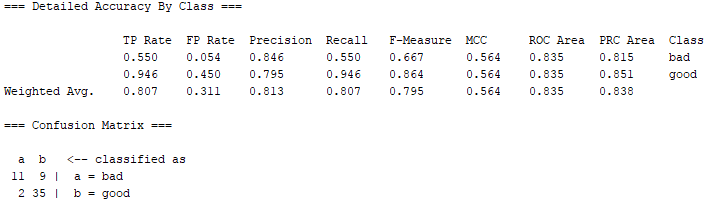
\includegraphics[scale=1]{2_6.png}
	\caption{Performance of Decision Stump on Labor Dataset.}
	\label{fig:PropProf}
\end{figure}

\subsubsection{Precision}
We can use the following formula to compute the \textit{Precision} out of the given confusion matrix. \textit{b} is considered as \textit{positive} and \textit{a} is considered as negative.
$$
PPV = \frac{TP}{TP + FP} = \frac{35}{35 + 9} = 0.79
$$

\subsubsection{Recall}
We can obtain \textit{Recall} of this classifier using the following formula.
$$
TPR = Recall = \frac{TP}{TP + FN} = \frac{35}{35 + 2} = 0.94
$$

\subsubsection{F1-Score}
F1-Score can be retrieved as follows. 
$$
F1_{score} = \frac{2 * PPV * TPR}{PPV + TPR} = \frac{2 * 0.94 * 0.79}{0.94 + 0.49} = \frac{1.4}{1.7} = 0.82
$$
\end{document}